% !TeX program = xelatex
\documentclass{csee}
% Use [fontset=fandol] on systems without the Windows fonts.
\usepackage{tikz} % Only used to draw the example figures.

\cseesetup{
  article-id = {待编},
  clc = {TM\hspace{0.25em}73},
  document-code = {A},
  subject-code = {470\hspace{0.25em}40},
  title = {电力系统同步相量测量算法的性能分析},
  authors = {张三\textsuperscript{1}，李四\textsuperscript{2}},
  affiliations = {（1．某某大学电气工程学院，北京市 100000；\\
    2．某某电力科学研究院，江苏省南京市 210000）},
  title-en = {Performance Analysis of Synchrophasor Measurement Algorithms\\
    for Power Systems},
  authors-en = {ZHANG San\textsuperscript{1}, LI Si\textsuperscript{2}},
  affiliations-en = {(1. School of Electrical Engineering, XX University, Beijing 100000, China;\\
    2. XX Electric Power Research Institute, Nanjing 210000, Jiangsu Province, China)},
  abstract-en = {This example demonstrates the layout of a bilingual paper.
    The title and author information span both columns. The abstract, main text,
    equations, figures, tables, and references are arranged in two columns.
    Replace the illustrative content with the results of your own research.},
  keywords-en = {power system; synchrophasor; measurement algorithm; performance analysis},
  abstract = {本文演示《中国电机工程学报》论文的基本排版，包括中英文题名、作者信息、
    摘要、关键词以及双栏正文。模板提供公式、双语图表题、参考文献、附录和作者简介的写法。
    文中数据仅用于展示格式，不代表实际研究结论。},
  keywords = {电力系统；同步相量；测量算法；性能分析},
  funding = {某某科研项目（项目编号）。},
  funding-en = {Project supported by the XX Research Program (Grant No. XX).},
  short-title = {张三等：电力系统同步相量测量算法的性能分析},
  % editor = {编辑姓名}, % Fill only if supplied by the journal.
}

\begin{document}
\maketitle
\makeabstract

\section{引言}
同步相量测量是电力系统监测的重要基础。撰写论文时，应在首次出现处说明符号与
缩略词的含义，统一变量的大小写、上下标和单位。文献引用使用连续编码，
例如文献\cite{ge2001,zhang2002}；图、表和公式分别连续编号。

正文采用五号宋体，英文和数字采用西文字体 Times New Roman，首行缩进为 0.74\,cm。
本示例展示主要排版接口，正式稿请替换作者、单位、基金项目和全部示例内容。

\section{方法与模型}
\subsection{信号模型}
设采样信号为 $x(t)$，幅值为 $A$，频率为 $f$，初始相位为 $\varphi$，则
\begin{equation}
  x(t)=A\cos(2\pi ft+\varphi).
  \label{eq:signal}
\end{equation}
式(\ref{eq:signal})中的变量使用数学斜体，单位使用正体。数值与单位之间保持
不可断开的四分之一字宽间距，如 \qty{12345.87908}{\micro\metre}。

\subsubsection{计算步骤}
\begin{enumerate}
  \item 采集原始信号并检查采样时间。
  \item 计算相量并统计测量误差。
\end{enumerate}
多行公式优先在关系符号处换行，符号留在上一行末：
\begin{equation}
  \begin{aligned}
    E ={}& (a_1+a_2+a_3) +{}\\
         & (b_1+b_2+b_3).
  \end{aligned}
  \label{eq:error}
\end{equation}

\begin{cseedefinition}[测量误差]\label{def:error}
测量值与参考值的差称为测量误差。
\end{cseedefinition}
\begin{cseetheorem}\label{thm:bound}
若各项误差均有界，则有限项误差之和有界。
\end{cseetheorem}

\subsection{算法性能比较}
表\ref{tab:comparison}给出原 Word 文档中的部分示例数据。表题置于表格上方，
顶线、底线为 0.75\,bp，栏目线为 0.5\,bp。
\begin{table}[htbp]
  \centering
  \cseecaption{DPMA与DFT算法的性能比较}
    {Performance Comparison Between DPMA and DFT Algorithms}
  \label{tab:comparison}
  \begin{tabular*}{\columnwidth}{@{\extracolsep{\fill}}lcccc@{}}
    \toprule
    算法 & $f_{\mathrm{sp}}/\mathrm{Hz}$ & $e_{\mathrm{ang}}/(^{\circ})$
      & $e_{\mathrm{mag}}/\text{‰}$ & $e_{\mathrm{TVE}}/\%$ \\
    \midrule
    DFT & 2 & \num{0.0997} & \num{2.1959} & \num{9.9716} \\
        & 3 & \num{0.1486} & \num{3.6945} & \num{14.8633} \\
    \midrule
    DPMA & 2 & \num{0.0073} & \num{1.2410} & \num{1.2381} \\
         & 3 & \num{0.0173} & \num{2.7717} & \num{2.7751} \\
    \bottomrule
  \end{tabular*}
\end{table}

\section{结果与讨论}
图\ref{fig:signal}演示单栏函数图。图中的数据曲线为主线，线宽为 0.75\,bp；
坐标轴为副线，线宽为 0.5\,bp。请使用矢量图或清晰的位图，并保证图中文字可读。
\begin{figure}[htbp]
  \centering
  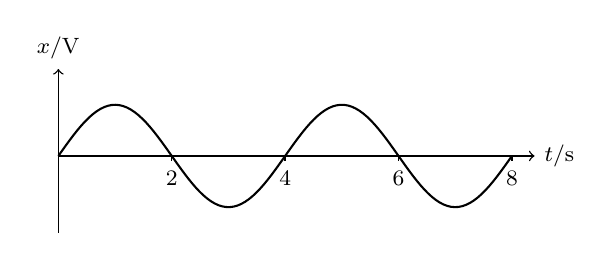
\begin{tikzpicture}[x=0.72cm,y=0.65cm,font=\fontsize{7.5bp}{10bp}\selectfont]
    \draw[line width=0.5bp,->] (0,0)--(8.4,0) node[right] {$t/\mathrm{s}$};
    \draw[line width=0.5bp,->] (0,-1.5)--(0,1.7) node[above] {$x/\mathrm{V}$};
    \foreach \x in {2,4,6,8} \draw[line width=0.5bp] (\x,0)--(\x,-0.1) node[below] {\x};
    \draw[line width=0.75bp,domain=0:8,samples=120] plot (\x,{sin(90*\x)});
  \end{tikzpicture}
  \cseecaption{采样信号示意图}{Illustration of the Sampled Signal}
  \label{fig:signal}
\end{figure}

数字应从小数点起每隔三位分组。使用 \verb|\num| 和 \verb|\qty| 可统一数字格式，
例如 \num{12345.87908} 和 \qty{50}{\hertz}。物理量的意义、单位与坐标轴方向应明确，
避免在不同章节中用同一个符号表示不同的量。

模板按原稿设置各级标题：一级为小四黑体，二级为五号黑体，三级为五号宋体。
希腊字母使用数学模式，例如 $\theta$、$\omega$、$\rho$ 和 $\Delta$。

\section{结论}
正文、图表、公式与参考文献应共同支持论文结论。此处填写研究结果、适用条件
及仍需解决的问题。删除未使用的示例环境和说明段落后，即可作为论文初稿使用。

\begin{cseeacknowledgements}
本文中实验方案的制定和实验数据的测量记录工作是在×××集团有限公司×××、
×××、×××等工作人员的大力支持下完成的，在此向他(她)们表示衷心的感谢。
\end{cseeacknowledgements}

% Manual entries retain the source document's GB/T 7714—2005 convention.
% Keep the bibliography in citation order; this environment does not sort it.
\begin{thebibliography}{99}
  \bibitem{ge2001}
  葛俊，童陆园，耿俊成，等．TCSC暂态过程中晶闸管导通角特性的研究[J]．
  电网技术，2001，25(7)：18-22．\par
  Ge Jun，Tong Luyuan，Geng Juncheng，et al．Research on thyristor conduction
  angle characteristics in transient process of TCSC[J]．Power System
  Technology，2001，25(7)：18-22(in Chinese)．
  \bibitem{zhang2002}
  张贤达．现代信号处理[M]．北京：清华大学出版社，2002：179-193．
\end{thebibliography}

\appendix
\section{补充说明}
附录采用小五号宋体、14\,bp 行距。附录中的图、表和公式按附录字母分别编号。
例如式(\ref{eq:appendix})与图\ref{fig:appendix}属于附录 A。
\begin{equation}
  y=kx+b.
  \label{eq:appendix}
\end{equation}
\begin{figure}[htbp]
  \centering
  \begin{tikzpicture}[font=\fontsize{7.5bp}{10bp}\selectfont]
    \draw[line width=0.5bp,->] (0,0)--(4.3,0) node[right] {$x$};
    \draw[line width=0.5bp,->] (0,0)--(0,1.8) node[above] {$y$};
    \draw[line width=0.75bp] (0.2,0.25)--(3.9,1.5);
  \end{tikzpicture}
  \cseecaption{简单函数示意图}{Illustration of a Simple Function}
  \label{fig:appendix}
\end{figure}

\par\addvspace{6bp}\noindent\textbf{作者简介：}
% For a real portrait use \begin{cseebiography}[portrait.jpg]{张三}.
\begin{cseebiography}{张三}
（1990—），男，博士，研究方向为电力系统测量与控制；
E-mail：\url{author@example.com}。
\end{cseebiography}
\begin{cseebiography}{李四}
（1992—），女，硕士，研究方向为电力系统运行与分析。
\end{cseebiography}
\cseeeditor
\end{document}
